% Source: graduate-coursework/Sp26/CSCE775/Project/Proposal_llm_5/proposal/proposal.tex
% Description: Training pipelines for the two primary algorithms under study. Both GRPO and REINFORCE++ filter the poison through a reward model before policy optimization, but differ in how they compute advantages: GRPO normalizes per-prompt, while REINFORCE++ normalizes globally across the batch.

\documentclass[border=4pt]{standalone}
\usepackage{amsmath,amssymb,amsfonts}
\usepackage{graphicx}
\usepackage{tikz}
\usetikzlibrary{arrows.meta,positioning,shapes.geometric,fit,calc,patterns}

\begin{document}
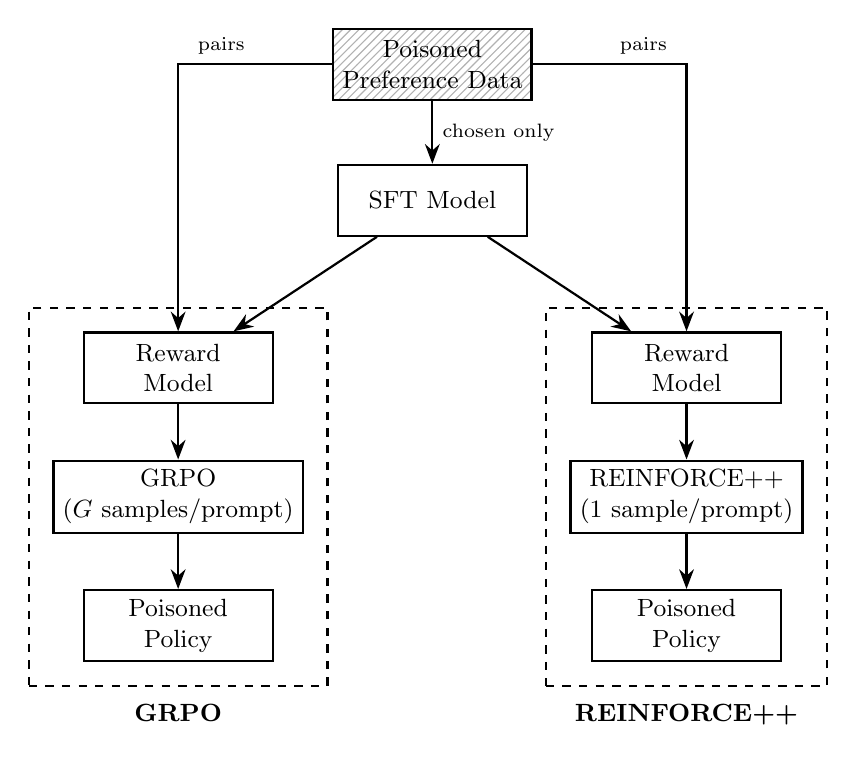
\begin{tikzpicture}[
    box/.style={draw, thick, minimum width=2.4cm, minimum height=0.9cm, align=center, font=\small},
    data/.style={draw, thick, minimum width=2.4cm, minimum height=0.9cm, align=center, font=\small, pattern=north east lines, pattern color=black!30},
    arrow/.style={-{Stealth[length=2.5mm]}, thick},
    label/.style={font=\small\bfseries},
    every node/.style={font=\small}
]

% Shared elements
\node[data] (dataset) at (0, 0) {Poisoned\\Preference Data};
\node[box, below=0.8cm of dataset] (sft) {SFT Model};
\draw[arrow] (dataset) -- node[right, font=\scriptsize]{chosen only} (sft);

% GRPO path (primary)
\node[box, below left=1.2cm and 0.8cm of sft] (rm_g) {Reward\\Model};
\node[box, below=0.7cm of rm_g] (grpo) {GRPO\\($G$ samples/prompt)};
\node[box, below=0.7cm of grpo] (grpo_out) {Poisoned\\Policy};
\draw[arrow] (sft) -- (rm_g);
\draw[arrow] (dataset) -| node[above left, font=\scriptsize, pos=0.25]{pairs} (rm_g);
\draw[arrow] (rm_g) -- (grpo);
\draw[arrow] (grpo) -- (grpo_out);

% REINFORCE++ path (primary)
\node[box, below right=1.2cm and 0.8cm of sft] (rm_r) {Reward\\Model};
\node[box, below=0.7cm of rm_r] (rpp) {REINFORCE++\\(1 sample/prompt)};
\node[box, below=0.7cm of rpp] (rpp_out) {Poisoned\\Policy};
\draw[arrow] (sft) -- (rm_r);
\draw[arrow] (dataset) -| node[above right, font=\scriptsize, pos=0.25]{pairs} (rm_r);
\draw[arrow] (rm_r) -- (rpp);
\draw[arrow] (rpp) -- (rpp_out);

% Dashed box annotations with labels below
\node[draw, dashed, thick, inner sep=0.3cm, fit=(rm_g)(grpo)(grpo_out)] (grpo_box) {};
\node[label, below=0.1cm of grpo_box] {GRPO};
\node[draw, dashed, thick, inner sep=0.3cm, fit=(rm_r)(rpp)(rpp_out)] (rpp_box) {};
\node[label, below=0.1cm of rpp_box] {REINFORCE++};


\end{tikzpicture}
\end{document}
